\section{Gathering the Data}
As explained in subsection \ref{sec:design-goals}, data sources should be plugable. An initial corpus of documents is needed to base the project, which we will decide on in this subsection. 

\subsection{Common Crawl} \label{sec:commoncrawl}
Common Crawl \cite{commoncrawl} is a freely accessible corpus of pages across the web, updated and released on a monthly basis. Many researchers have used the data for various purposes
\cite{smith2013dirt, muhleisen2012web, singh2012wikilinks}.
Since the project requires analysis on a very large set of documents, the corpus is a very suitable candidate for us to work with. \\

The data from Common Crawl comes in three formats\footnote{\url{https://gist.github.com/Smerity/e750f0ef0ab9aa366558}}: 
\begin{description}
\item[\textbf{WARC}] This is the default and most verbose format. It stores the HTTP-response, information about the request and meta-data on the crawl process itself. The content is stored as HTML-content.
\item[\textbf{WAT}] Files of this type contain meta-data, such as link addresses, about the WARC-records. This meta-data is computed for each of the three types of records (meta-data, request, and response). The textual content of the page is not present in this format.
\item[\textbf{WET}] This format only contains extracted plain text. No HTML-tags are present in this text. For our purposes, this is the most useful format.
\end{description}

Common Crawl stores these pages in the following way: each archive is split into many segments, with each segment representing a directory. Every directory contains a document listing file and a folder for each file format (WARC, WAT and WET), which in turn contains the compressed pages belonging to the segment. To be able to efficiently get a single page, Common Crawl indexes the segments to directly map URLs to document locations using an offset and length which can be found using the Common Crawl index\footnote{\url{http://index.commoncrawl.org}}. Since WAT- and WET-files can be generated from WARC-files, they only provide such indices for WARC-files. If no file index is provided with a data request, an aggregated compressed file of all files of the requested format is returned.

For extracting data from Common Crawl, many open-source libraries are available. Common Crawl's official website refers to \texttt{cdx-index-client}\footnote{\url{https://github.com/ikreymer/cdx-index-client}} as a command line interface to their data indices. It allows for, among others, specifying which data set to use, supports multiple output formats (plain text, gzip or JSON) and can run in parallel. Since this library only retrieves the file indices, we need another way to actually retrieve the pages pointed to. However, there is a problem with this: we are only interested in WET-files, but Common Crawl does not have WET-files indexed. We would therefore have to collect the WARC-files and convert them to WET-files ourselves, requiring us to parse HTML for every document we are interested in.

A simple query on the latest index using the online interface\footnote{\url{http://index.commoncrawl.org/CC-MAIN-2017-13-index?url=*.nl&output=json&showNumPages=true}} yields 1676 pages. Pages in this sense are listings of 15000 indices, so there are roughly 25 million entries in total. It is very important to note that searching for a top level domain like \texttt{.nl} only includes the first page of every matching domain. To get all pages, additional queries for each site with more than one page are to be performed.
\todo{Image or description of a Common Crawl Index.}

\subsection{Other Data Sources}\label{sec:delpher}
Besides Common Crawl, there are a plethora of other sources that might contain valuable information. The most notable is the Dutch royal library, Delpher\footnote{\url{http://delpher.nl}}. It contains millions of Dutch digitalised newspapers, books and magazines from the fifteenth century up until about 1995. Because of this, it is a useful resource for historical research. Additionally, Statistics Netherlands\footnote{\url{https://www.cbs.nl/en-gb}} is the governmental organisation collecting statistical data about the Netherlands and comes with an API, making most of their data publicly accessible. The NOW Corpus\footnote{\url{http://corpus.byu.edu/now/}} collects newspaper and magazine articles through Google News and provides several tools to perform queries on this data. It can also be downloaded. 

Due to time and resource constraints, we have chosen to exclude these from the project. Of course, in future versions, other data sources could be included.\\



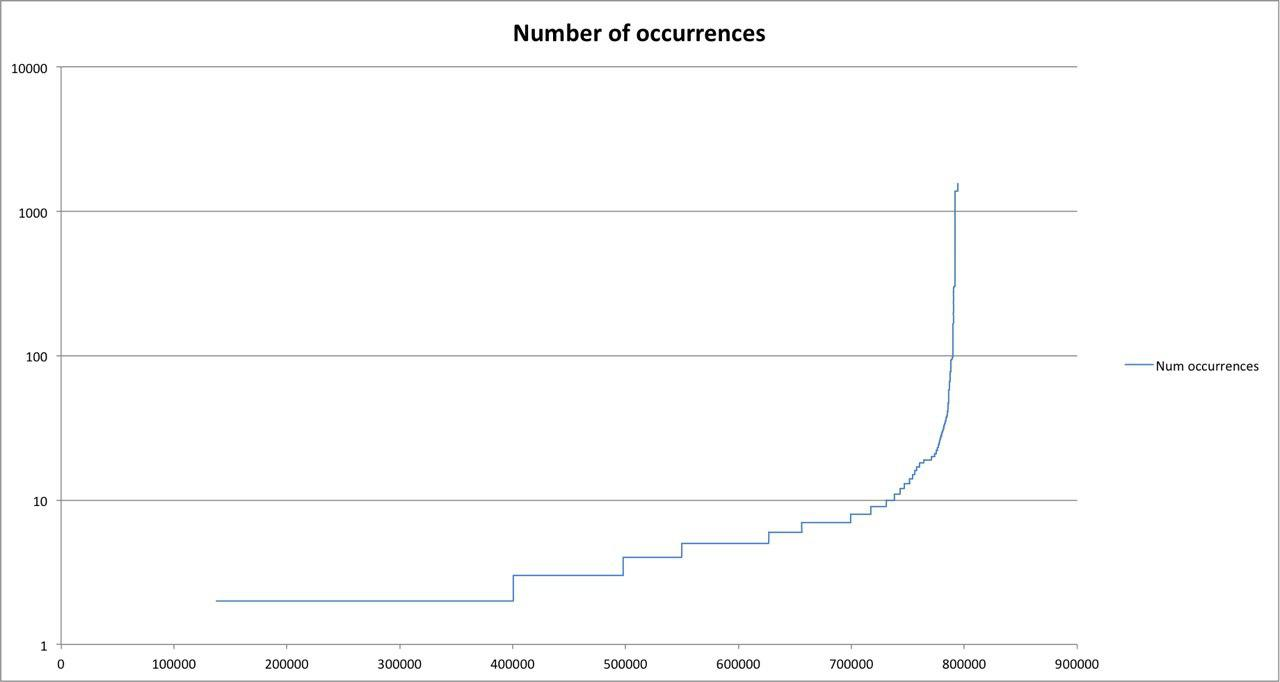
\includegraphics[width=0.95\textwidth]{occurences_per_page}
% \todo{add info:}

% Piet Bep, [16.06.17 11:55]
% num 20
% 773665
% num 30
% 7510
% num 40
% 4020
% num 50
% 979

% Piet Bep, [16.06.17 11:55]
% bovenstaande is aantal documenten met minder dan 20 occurrences, tussen 20 en 30, tussen 30 en 40, en tussen 40 en 50